
\section{RobotCub and ICub}
RobotCub is a collaborative project funded by the European Commission under 
the Framework 6 program and it is part of the Cognitive Systems effort 
coordinated by the Unit E5 \cite{e5-cognition}.
One of the goals of RobotCub is that of creating an open platform where
many other projects could thrive by exploiting a common hardware and software
infrastructure. RobotCub has also the goal of making the {\em ICub} (this is 
the name of the robot) the platform of choice for several other research
groups worldwide and, simultaneously, to advance our knowledge of natural and
artificial cognitive systems.

One of the tenets of the RobotCub stance on cognition is that manipulation 
plays a key role in the development of cognitive capability. Consequently, 
the design is aimed at maximizing the number of degrees of freedom of the upper 
part of the body (head, torso, arms, and hands). The lower body (legs) is made 
to support crawling on the four limbs and sitting on the ground in a stable 
position with smooth autonomous transition from crawling to sitting. This  
allows exploration of the environment, grasping and manipulation of objects 
lying on the floor. The total height is estimated to be around 105cm. The 
total number of degrees of freedom (DOF) is 53 of which 41 in the upper body 
(7 for each arm, 9 for each hand, 6 for the head and 3 for the torso and spine). 
Each leg consists of six additional degrees of freedom. The sensory system will 
include binocular vision and haptic, cutaneous, aural, and vestibular sensors.
We cared particularly in placing the sensors as in the human body and consequently 
there are two moving eyes with cameras, two microphones surrounded by pinnae, the
inertial sensing is located in the head and tactile sensors are planned to cover 
as much as possible of the robot body. Each joint is also equipped with position
and temperature sensors (for safety of operation). There are plans for adding 
joint-level torque measurement and eventually implement force/impendance control.
Functionally, the system should be able to coordinate the movement of the eyes 
and hands, grasp and manipulate lightweight objects of reasonable size and 
appearance, crawl using its arms and legs, and sit up. This allows the system 
to explore and interact with the environment not only by manipulating objects 
but also through locomotion.

\begin{figure}[tbp]
\centerline{
\includegraphics[width=\textwidth]{fig-icub}
}
\caption{The ICub at various stages of construction. Panel A) shows the head
of the robot with part of the embedded electronics and sensors; in B) the upper
torso showing also the left hand; C) shows a first realization of the legs (now
improved); D) a tentative assembly of the entire robot, showing its scale; 
E) a more recent assembly, showing the robot supporting its own weight
passively.
} 
\label{fig:icub}
\end{figure}


The philosophy adopted by RobotCub is that of
the free software movement,
as codified by the General Public License (GPL). 
On the software side, the RobotCub project adopted YARP and contributed
to the development of some new specific features. For the hardware, we
selected the GPL license for the sources and FDL for documentation
and drawings. While it is clear how to apply these licensing
schemes to source code (e.g. C++), we need to clarify how to
apply them also to hardware designs.

\subsection{Open Source hardware}
The phrase ``Open Source hardware'' might sound strange,
 but in fact it is a 
plain transfer of the open source philosophy to the entire
design of the RobotCub platform.
%
%
The design of the robot started from 
the preparation of specifications (e.g. estimation of torque, speed, etc.),
a typical 3D CAD modeling, and eventually in the preparation
of the executive files which are used to fabricate parts and for assembly. 
Without good documentation it is very complicated to build and assemble 
a full robot. This means that documentation (as for software) is particularly 
important.

The CAD files, in some sense, can be seen as the source code, since
they are the ``preferred form of the work for making modifications
to it'', in the language of the GPL.
%
They get ``compiled''
into 2D drawings which represent the executive drawings that can be used by any
professional and reasonably well-equipped machine shop either to program CNC machines 
or to manually prepare the mechanical parts. This compilation process is not fully 
automated and requires substantial human intervention. There is a clear dependency 
of the 2D drawings on the original 3D CAD model. To enable the same type of virtuous 
development cycle as occurs in open source software, the 3D CAD is required, since changes happen 
in 3D first and get propagated to 2D later. In addition, assembly diagrams, part 
lists, and all the material produced during the design stage should be included 
to guarantee that the same information is available to new developers.


One difference between software and the hardware design is that there are
currently no effective formats for interchange of 3D models.
%
Proprietary systems such as SolidWorks and Pro/E can import and export
a range of formats, but going from one to another is lossy, destroying
information needed for production and leaving just the basic geometrical
shape.
%
So in practice, designs are tied to tools produced by a particular
vendor, and interoperability
between hardware design tools is limited.
%
% The equivalent of an approximately portable language like C++ 
%does not exist in this case. 
%
%While this might not be seen as an advantage in practice
%it eases the preparation of the standards. 
%
In RobotCub we were forced to choose a specific 
set of tools for mechanical and electronic CAD and future upgrades will have to strictly 
adhere to these standards. 
%
Due to the absence of open source professional design tools, RobotCub
uses proprietary products. 
%
This is an unfortunate situation, but there is no practical
alternative at the moment.  The ``C++'' and ``gcc'' of 
CAD do not yet exist.
%

As a practical matter, the simple duplication of RobotCub parts does not
require the use of any of these tools since we provide all executive drawings and 
production files (e.g. Gerber files for the PCBs).
%
%
%Due to the absence of open source professional design tools, RobotCub
%uses proprietary products. 
%
For modification, the design tools are somewhat expensive
(educational discounts or educational releases exist).
Free of charge {\em viewers} are
currently available for all file types in question. 
%

For RobotCub, we decided to license all the CAD sources under the GPL
which seems appropriate given their nature.  Associated documentation
will be licensed under the FDL.  These will be made available through
the usual source code distribution channels (e.g. repositories,
websites).

Another difference with respect to GPL on software is that the cost
of duplication is significant and variable. Copying and duplicating 
software has a negligible cost and the copy is as functional as the 
original. To copy the hardware requires access to a well-equipped
machine shop and to specialized machines for fabrication of the 
electronics. The process of assembling the parts is also non-trivial
with possibly additional use of special tools and machining. 
Copying software is almost error-free, hardware incurs in additional 
cost related to mistakes and parts that needs to be brought within 
specs.

\subsection{The design process}
The design process of RobotCub has been a distributed effort as for many open
source projects. Various groups developed various subcomponents and contributed in
different ways to the design of the robot including mechanics, electronics, sensors, 
etc. In particular, a whole design cycle was carried out for the subparts (e.g.
head, hand, legs) and prototypes built and debugged. The final CAD and 2D drawings 
were discussed and then moved to the integration stage. Clearly, communication
was crucial at the initial design stage to guarantee a uniform design and a
global optimization.

The distributed design broke down at the integration stage where the industrial 
partner\footnote{Telerobot Srl, Genoa} stepped in to carry out integration, 
verification and consistency checks. The design and fabrication of the control 
electronics was also subcontracted to a specialized company.
It is important to stress the collaboration with industry for a project of this
size and with these goals and requirements. For many reasons building a complete 
platform involves techniques and management that is better executed by applying 
industrial standards. One example that applies to RobotCub is the standardization 
of the documentation.

A further strategy used in RobotCub is that of building early. Each subsystem
was built as soon as possible and copied also as soon as possible. In several cases
debugging happened because the copies of the robot did not work as expected or
easy to fix problems were spotted. Sometimes the documentation had to be improved.
Unfortunately, this strategy was applied less extensively to some of the subparts 
which are or were still under design and debugging. 

The design stage will be completed by the realization of ten copies of the ICub.
This will further test the documentation and in general the reliability of the
overall platform including software, debugging tools, electronics, etc. The first
release of the ICub will be consolidated after this final fabrication stage.

The actual design of the robot had to incorporate manipulation by providing 
sophisticated hands, a flexible oculomotor system, and a reasonable bi-manual 
workspace. On top of this, the robot has to support global body movements such as 
crawling, sitting, etc. These many constraints were considered in preparing 
the specifications of the robot and later on during the whole design process.

The behaviors we set forward for representing the robot's skills generate two 
types of constraints:
\begin{itemize}
	\item kinematics: about the geometrical construction of the robot;
	\item dynamics: about the forces and torques we require from the robot.
\end{itemize}

The possibility of achieving certain tasks is favored by a suitable kinematics, 
and in particular this translates into the determination of the range of movement 
and the number of controllable joints (where clearly replicating the human body 
in detail is impossible with current technology). Kinematics is also 
influenced by the overall size of the robot. We decided {\em a priori} to target the 
size of a three and a half year old child (approximately $1m$ tall). Actual 
dimensions were taken from studies in ergonomics and x-ray images \cite{tilley01measure}. 
This size can be achieved with current technology. QRIO \cite{sony-qrio} is an example 
of a robot similar in size although with less degrees of freedom. In particular, 
our specifications had to consider hands and moving eyes. Also, we wanted to 
consider the workspace and dexterity of the arms and thus a three degree of 
freedom shoulder was a requirement. 

%Later, we will elaborate these considerations into a proper list of joints, 
%ranges, and sensory requirements at the joint level.

Considering dynamics, the most demanding requirements appear in the 
interaction with the environment. Impact forces, for instance, had to be 
considered for the crawling behavior, but also and more importantly, developing 
cognitive behaviors such as manipulation might require exploring the environment 
erratically. As a consequence, it is likely that impacts will occur with
various parts of the robot structure. This turns out to require strong 
joints, gearboxes, and powerful actuators or alternatively
passive compliance and soft materials. In order to evaluate 
the scale (order of magnitude) of the required forces we ran simulations 
of various behaviors in a reasonable model of the robot. These dynamic simulations 
provided data for starting the design of the robot.

At a more general level we had then to evaluate the available technology, compared 
to the experience of the RobotCub consortium and the targeted size of the robot: 
it was decided that electric motors represent the most suitable technology for 
the ICub, given also that it has to be ready according to a very 
tight schedule in the span of the RobotCub project. Other technologies 
(e.g. hydraulic) are left for a ``technology watch'' activity and they were 
not considered further.

In addition, given the size of the robot, and given the power density available, 
considerations of speed for certain joints lack significance: i.e. given the 
power and the torques required, speed is a consequence rather than a design 
parameter. In certain cases, in comparing to human data, clearly also the power 
density is much lower than desired (e.g. the wrists cannot possibly support the weight 
of the robot).

Finally, the ICub is not only about motors, sensors are equally important. 
Also in this case, we had to deal with and exploit  the available technology as best we could. 
The robot has vision, audition, joint sensors, force sensors, tactile 
sensors - where possible - and temperature sensors in many of the motors. The robot 
can give feedback through a speaker. ICub will thus include a plethora of sensors as
cameras, microphones, gyroscopes, linear accelerometers, encoders (or other positional
sensors), temperature and current consumption sensors, force/torque, and tactile
sensors. The choice of these components is clearly related to the robot specifications.

To recapitulate, the constraints of size and available technology determine a good 
part of the design choices - i.e. our freedom in deciding which components to use. 
In parallel, we simulated some of the robot's behaviors to determine the required 
joint torques. These two pieces of information were then used in selecting the best 
available motors compatible in size, torque, and strength. As we mentioned earlier, 
speed is a consequence rather than a design parameters here, although, in simulation we 
examined the dependency of speed to torque for crawling.

Other design choices are related to the embedded electronics and the structure of 
the software. The ICub will have many sensors and actuators working in parallel. We 
would like to exploit this parallelism also at the computational level and, consequently, 
the ICub API was mapped one-to-one onto YARP.

\subsection{Modularity}
The ICub design is modular across two dimensions, namely, the mechanical hardware
and the control structure. Mechanically, the robot has a certain degree of modularity
which allows for improvements without a full-blown redesign activity. The controller
is modular in the sense that it is made of several layers. Each layer can be replaced
with a different technology and/or implementation without much suffering.

When we consider hardware modularity, we need to strike a balance
between the desirability of a global optimization and the advantages of modular and 
dependable design. The current design probably reflects more the desire
to achieve certain functionalities, within a given size, in a constrained setting of three 
years dedicated to design rather than the search for the quality and maintainability 
of the robot in the long term. In essence, the ICub is and will remain a research 
platform. It cannot be considered akin to the AIBO, nor a more industrial realization 
like the HRP2.

In spite of these stringent requirements the ICub shows modularity and macro-subgroups
can be identified in the hand plus forearm, in the arm (entire arm), in the head, the torso,
and the legs. These parts can be built and maintained, developed, and assembled 
separately. Finer grained modularity is not possible because of the placement of the
motors and the routing of the tendons. The electronics represent another element of
complication since the control cards for certain groups are not localized within the 
groups (e.g. the hand controllers are in the upper arm section).

Assembly techniques have been considered for mechanical parts and details have been
optimized to favor mechanical realization (e.g. tendon routing has been considered and
the assembly sequence optimized whenever possible). Nonetheless the realization 
of the hands (the most complicated parts of the robot) requires considerable time 
and effort.

\begin{figure}[tbp]
\centerline{
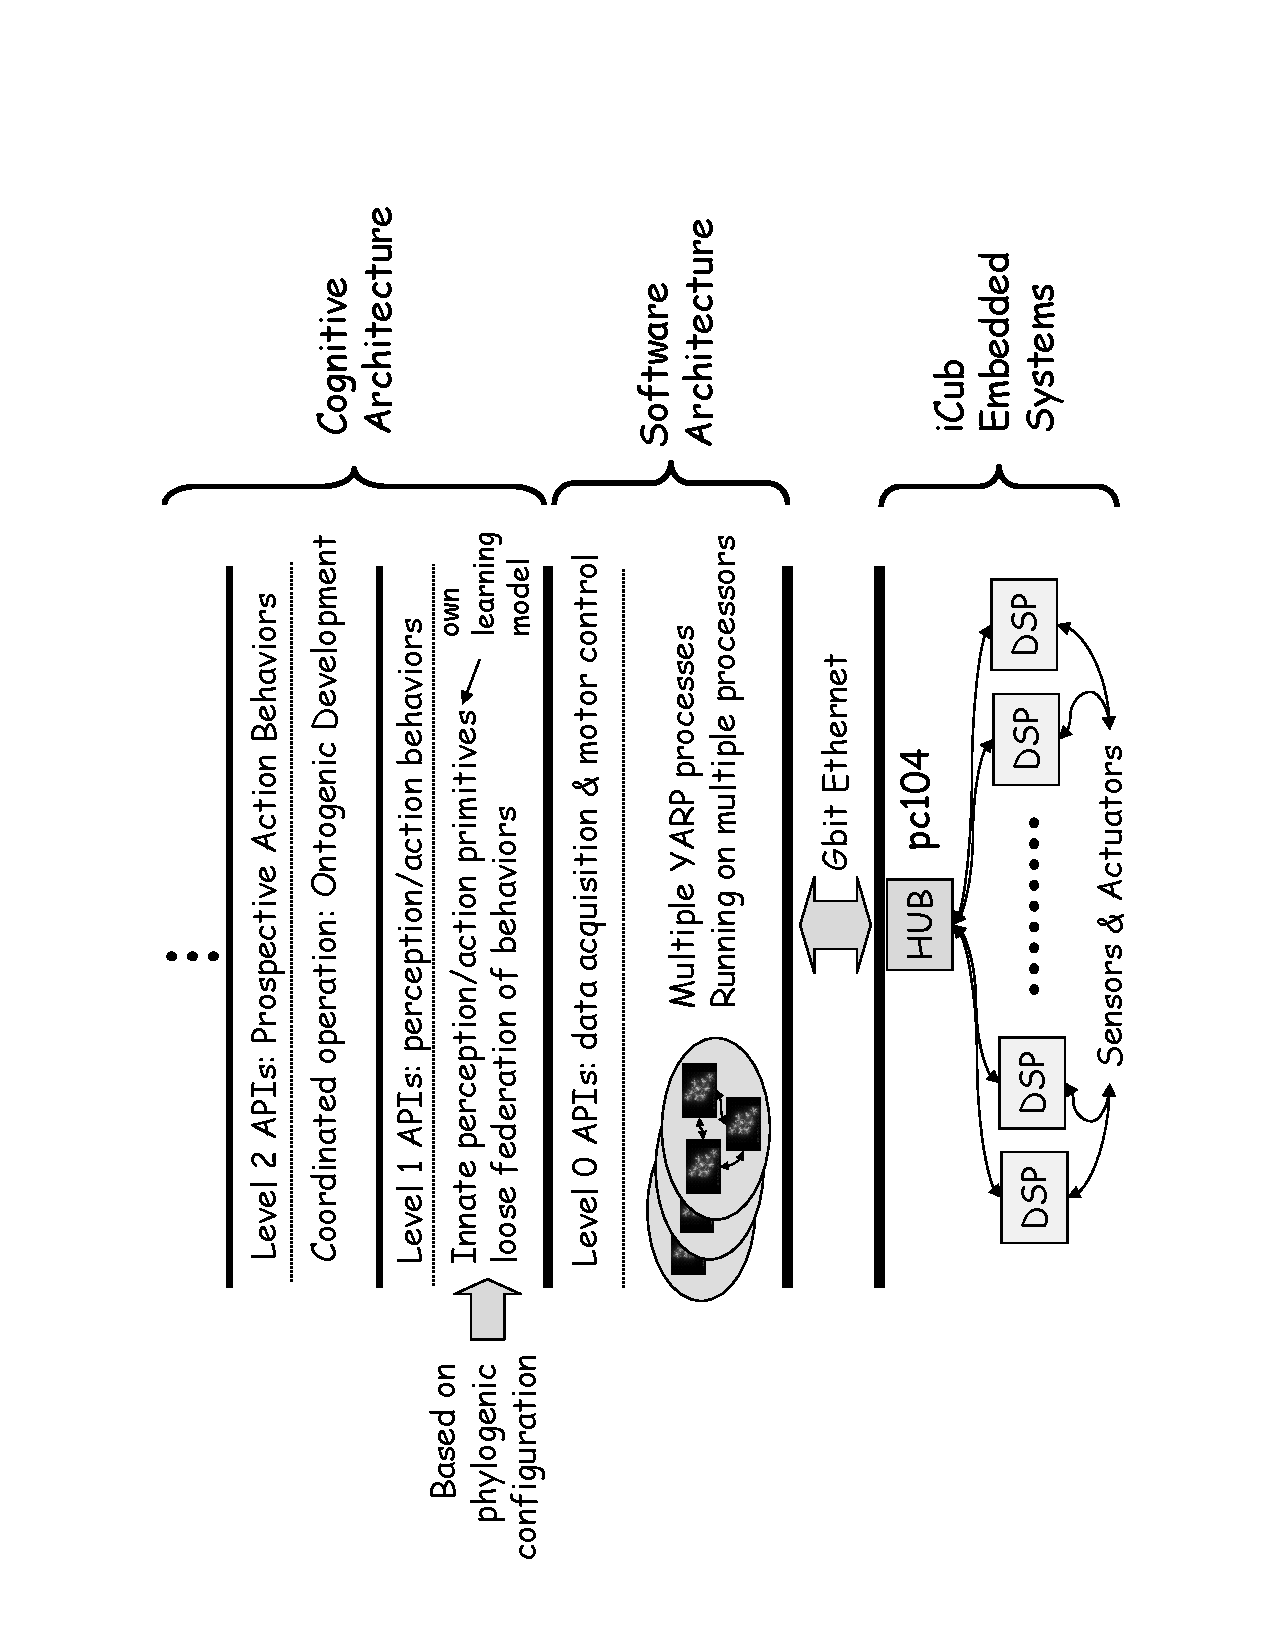
\includegraphics[width=15cm]{layers}
}
\caption{The layered structure of the ICub. The lowest level is the DSP layer which 
directly connects to the motors and/or sensors. The next hardware level is represented
by the PC104 HUB which interfaces on one side to all data sources and controllers and
on the other to the GBit Ethernet network. The next layer is a distributed computation
engine made of a set of standard PCs which communicate through YARP. On top of this
the RobotCub partners will develop a cognitive architecture. Communication is defined by
protocols as for example, from the DSP to the motors, from the PC104 to the DSP, and from
the YARP processes to the PC104. Standardization at this level favors reusability and
dependability of the system.} 
\label{fig:layers}
\end{figure}

At the controller level, modularity is described by at least three layers:
\begin{itemize}
	\item the DSP-controller level;
	\item the HUB-coordination level (interface);
	\item the control architecture.
\end{itemize}
The DSP level consists of a set of controller cards that can drive the motors
directly but also by virtue of programmability enable the preparation of local
sophisticated control algorithms. These controller cards were specifically 
designed for the ICub. They communicate through a set of four CAN bus backbones
to a Pentium-based HUB card which can do both synchronization of sensorial and
motoric data and run simple control loops in case they are needed to be local 
to the hardware (for very tight timing). The Pentium, a PC104 format CPU card, is 
interfaced to YARP processes through a Gbit Ethernet cable.
The interface at this level is fully YARP-compatible and specified at the level
of ports or device drivers. The YARP processes form the control architecture 
and can implement complex cognitive behaviors (as indicated in Figure \ref{fig:layers}).

Protocols are specified at each level. Electrical between the controllers and the
motors (determined by the motor specifications), software and electrical (CAN) 
between the DSP and the PC104 HUB, also software at the level of the YARP 
packets that travel on the GBit Ethernet cable, and clearly software between 
the modules of the cognitive architecture. 
Replacement of components, as long as the protocols remain unchanged, is likely
to require only the redesign of the appropriate layer. For example, the obsolescence 
of the DSP microcontroller currently in use may lead to a new version that can 
be made compatible with the current CAN bus specification. 



\begin{figure}[tbp]
\centerline{
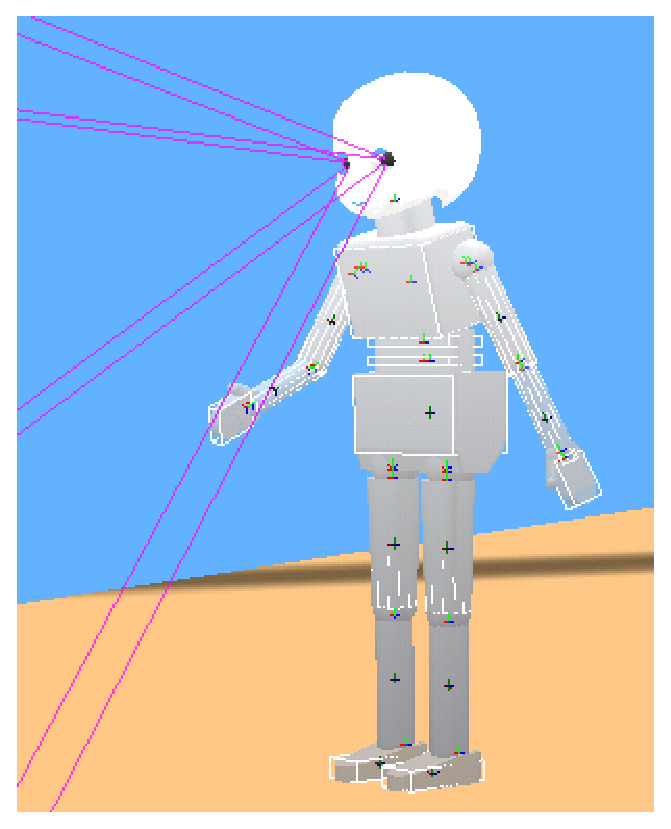
\includegraphics[height=6cm]{sim-webot-detail}
}
\ \\
\centerline{
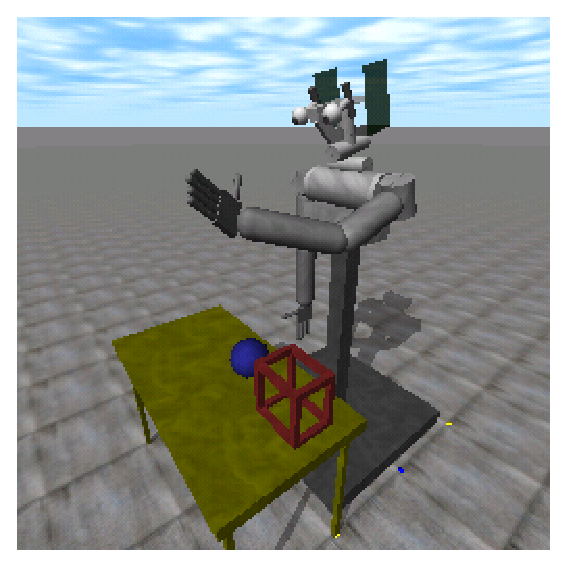
\includegraphics[width=3.5cm]{sim-ode-wide} 
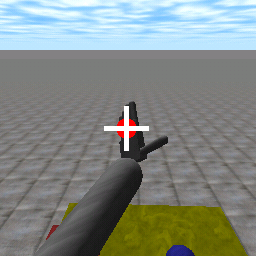
\includegraphics[width=3.5cm]{sim-ode-left} 
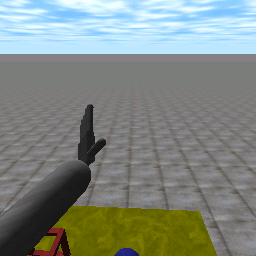
\includegraphics[width=3.5cm]{sim-ode-right}
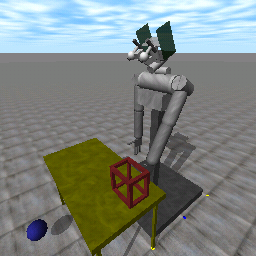
\includegraphics[width=3.5cm]{sim-ode-knock}
}
\caption{
%
The ICub robot has two simulators.
One uses the (propietary) Webots package, and the other uses
the Open Dynamics Engine (ODE) library directly.
The Webots interface is shown in the top image, and is currently
the most complete simulation.  The ODE simulation (lower row)
is currently of the robot's upper torso.  Shown from left to
right: the ICub simulation tracking its hand visually;
the view from the ``dominant'' camera used for tracking; the
view from the non-dominant camera; the robot arm hitting
a table, causing the blue ball to roll off.
%
See the acknowledgements section for simulator author credits.
%
The two simulators and the actual robot have the same interface either
when viewed via the device API or across network, and so
are all more or less interchangeable from a user perspective.
%
%So it is possible to control any of the robots from a program using the
%same device or network interfaces.  
%
There are of course
differences in the detailed behavior of all three, which we hope to
reduce over time.
%
} 
\label{fig:simulators}
\end{figure}

%% It is also possible to control the robots
%% without using any YARP or ICub code, just elementary TCP and text
%% messages.  To read images from the cameras, it would be more
%% efficient to do a little extra study to understand binary mode
%% operation, since the bandwidth is large enough to make the extra cost
%% of text-mode operation non-negligible.  Of course we expect YARP and
%% ICub libraries to be used (that's why we're writing them)
